\section{Modello di Ising 2D}

Il modello di Ising 2D è un reticolo quadrato bidimensionale di spin che possono assumere solamente i valori $\pm 1$. L'Hamiltoniana 
del sistema è la stessa riportata in precedenza

\begin{equation}
    H\,=\,-J\sum_{\left<ij\right>} \sigma_i \sigma_j\,-\,h\sum_{i} \sigma_i,
    \label{eq: ising2D_ham}
\end{equation}

con la differenza che in questo caso ogni momento magnetico presenta quattro primi vicini. Il modello presenta soluzione analitica 
solamente nel caso di campo magnetico nullo. In tali condizioni, la magnetizzazione risulta essere 

\begin{equation}
    m\left(\beta,\,h=0\right)\,=\,
    \begin{cases}
    \left[1\,-\,\dfrac{1}{\sinh^4{\left(2\beta J\right)}}\right]^{\frac{1}{8}} \qquad \qquad T\,<\,T_c \\
    0 \qquad \qquad \qquad \qquad \qquad \qquad \,\,\,\, T\,>\,T_c.
    \end{cases}
    \label{eq: magn_Onsager_1944}
\end{equation}

dove $T_c$ è pari a 

\begin{equation}
    T_c\,=\,\frac{2J}{\ln{\left(1\,+\,\sqrt{2}\right)}}.
    \label{eq: tc_Ising2D_Ons}
\end{equation}

Come risulta evidente in Figura \ref{fig: magn_Ising2D}, la magnetizzazione passa rapidamente da un valore unitario a zero nell'intorno 
della temperatura critica. Dato che la magnetizzazione costituisce il parametro d'ordine per il modello di Ising, questo comportamento è
un'evidenza della transizione di fase che il reticolo di spin subisce.

\begin{figure}[H]
    \centering
    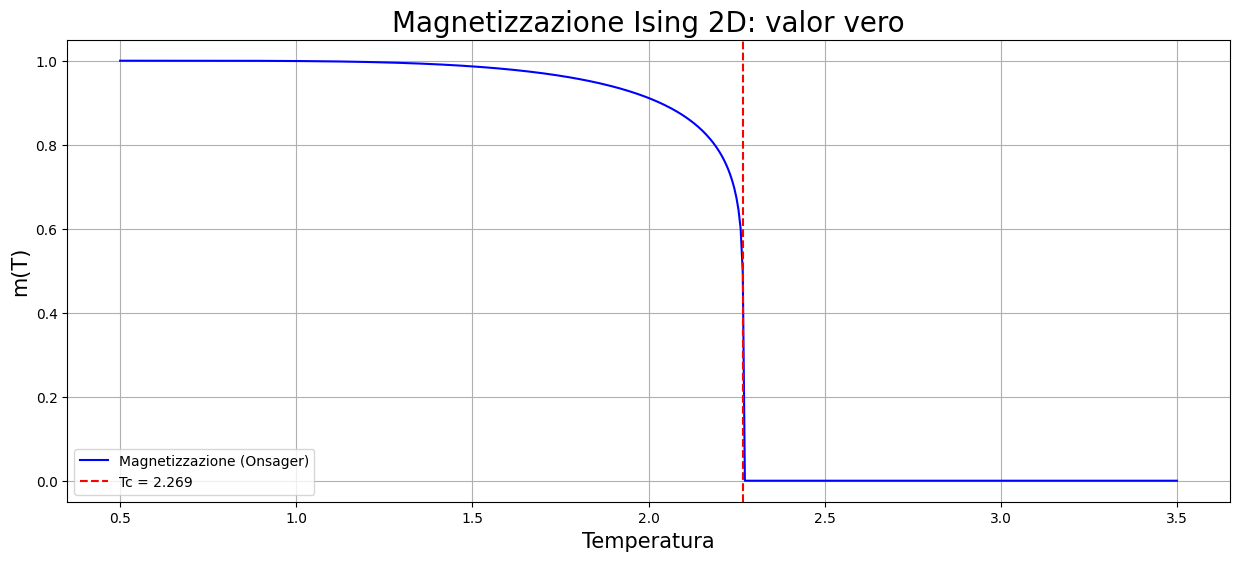
\includegraphics[width=\textwidth]{Immagini/magn_Ising2D.png}
    \caption{Magnetizzazione per il modello di Ising 2D in assenza di campo magnetico. E' possibile osservare come a $T\,=\,T_c$ la 
    magnetizzazione passa rapidamente da un valore unitario a zero. }
    \label{fig: magn_Ising2D}
\end{figure}

Al di sopra della temperatura critica il sistema è di natura paramagnetica e la magnetizzazione è nulla. Invece per $T\,<\,T_c$ gli 
spin sono ordinati ed il sistema presenta magnetizzazione spontanea. Per quanto riguarda l'energia interna, essa 
è data da \cite{Patria}

\begin{equation}
    U\,=\,-NJ\coth{\left(2\beta J\right)}\left\{1\,+\,\frac{2}{\pi}\left[2\tanh^2\left(2\beta J\right)\,-\,1\right]\int_0^{\pi/2}\frac{d\phi}{\sqrt{1\,-\,k^2\sin^2{\left(\phi\right)}}}\right\},
    \label{eq: ene_Onsager_1944}
\end{equation}

dove $k\,=\,2\sinh{\left(2\beta J\right)}/2\cosh^2{\left(2\beta J\right)}$ e l'integrale che compare nella relazione 
precedente è un integrale ellittico completo del primo ordine.



\subsection{Finite size scaling}

I modelli su cui è possibile effettuare uno studio computazionale hanno dimensione finita e di conseguenza sono solo un'approssimazione 
del limite termodinamico; il fatto che non venga considerato un numero di spin infinito si traduce in una descrizione inesatta della 
transizione di fase. Per $T \to T_c$ la lunghezza di correlazione dovrebbe divergere, ma per un sistema come quelli simulati per mezzo di 
tecniche Monte-Carlo, il massimo valore di $\xi$ è $L$, ossia la dimensione lineare del reticolo. A causa di questo cut-off sulla 
lunghezza di correlazione, altre quantità divergenti come il calore specifico e la suscettività magnetica presenteranno semplicemente un 
picco a $T_c$, ma non assumeranno valore infinito. Inoltre la caduta della magnetizzazione non sarà tanto rapida come per il risultato 
analitico, ma invece di un gradino si otterrà una curva derivabile in cui $m$ tende a zero meno rapidamente. La temperatura critica, 
che per il modello di Ising 2D è $T_c \simeq 2.269$, non può essere predetta correttamente simulando un sistema finito. Supponendo di 
avere un reticolo di dimensione $L$, la temperatura critica valutata con un analisi computazionale differisce da quella calcolata 
analiticamente nel limite termodinamico di un fattore che dipende proprio dalla size del sistema. Infatti 

\begin{equation}
	T_c\left(L\right)\,-\,T_c\left(\infty\right) \simeq L^{-1/\nu}
	\label{eq: fs_Tc}
\end{equation}

Questo risulta evidente nello studio del calore specifico al variare della temperatura critica riportato in Figura \ref{fig: cp_Ising2D_crit}, in cui il 
picco dello stesso tende al valor vero all'aumento della dimensione reticolare.

\begin{figure}[H]
    \centering
    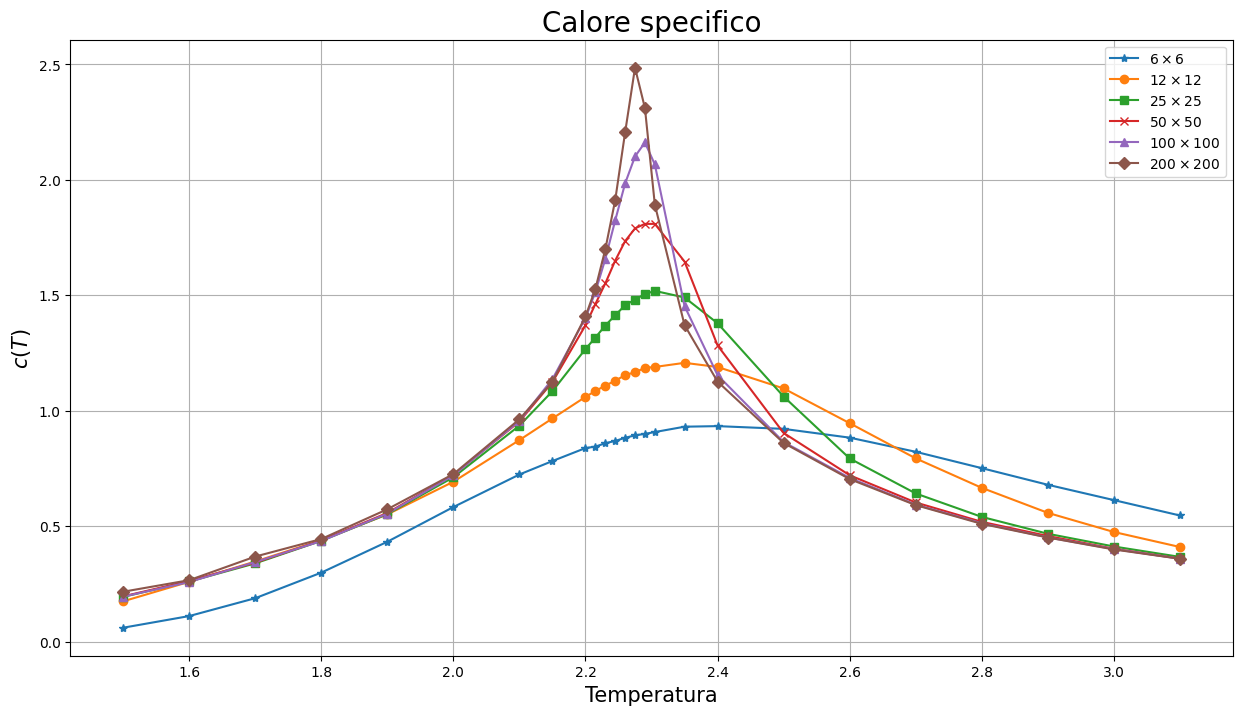
\includegraphics[width=0.9\textwidth]{Immagini/simIsing2D/cp.png}
    \caption{Calore specifico: h = 0.0.}
    \label{fig: cp_Ising2D_crit}
\end{figure}


\subsection{Domain walls}

Consideriamo ora un sistema di dimensione lineare $La$, dove $L$ è un numero reale ed $a$ invece il passo reticolare, in uno spazio a $d$ dimensioni. 
Supponiamo inoltre che tale reticolo presenti un domain wall. In analogia con quanto osservato per il modello di Ising 1D, la 
variazione di energia legata a questa struttura è pari a 

\begin{equation}
    \Delta E\,=\,2JL^{d-1}
    \label{eq: ene_dw_IsingdD}
\end{equation}

L'entropia del domain wall è legata al numero di modi in cui si può costruire tale interfaccia. Per un singolo domain wall si può 
stimare che 

\begin{equation}
    S \gtrsim k_B \ln{\left(L\right)}
    \label{eq: entr_dw_IsingdD}
\end{equation}

L'energia libera associata alla presenza dell'interfaccia è dunque pari a 

\begin{equation}
    A \simeq 2JL^{d-1}\,-\,k_B T\ln{\left(L\right)},
    \label{eq: freeE_dw_IsingdD}
\end{equation}

che è dominata dal termine energetico per ogni dimensione maggiore di due, dato che nel limite termodinamico il termine 
logaritmico è trascurabile. Per provare l'esistenza di ferromagnetismo in modo più quantitativo, basta mostrare che il valor medio 
dello spin sia diverso da zero. Nel caso del modello di Ising 2D è possibile mostrare che se gli spin che fanno parte della cornice 
esterna del retico sono positivi, la probabilità di avere uno spin negativo al centro del sistema è pari a 

\begin{equation}
    p_{-}\,<\,\frac{1}{2}\frac{\exp{\left(-2\beta J\right)}}{4 \left(1\,-\,3\exp{\left(-2\beta J\right)}\right)^4}.
    \label{eq: probm_Ising2D}
\end{equation}

Il secondo membro della relazione \eqref{eq: probm_Ising2D} può essere reso minore di $1/2$ in modo indipendente dalla dimensione del reticolo 
(ossia del parametro $L$ introdotto in precedenza) scegliendo una temperatura opportuna. Questo evidenzia come possa 
presentarsi long range order e di conseguenza magnetizzazione finita per $0\,\leq T\,<\,T_c$. Per sottolineare ulteriormente le 
differenze fra il modello di Ising 1D e quello bi-dimensionale consideriamo ora il mapping riportato in Figura \ref{fig: map_2to1_Ising}, 
in cui i siti reticolari di un modello bi-dimensione vengono mappati su una catena lineare (mantendo l'interazione con i primi 
vicini di partenza).

\begin{figure}[H]
    \centering
    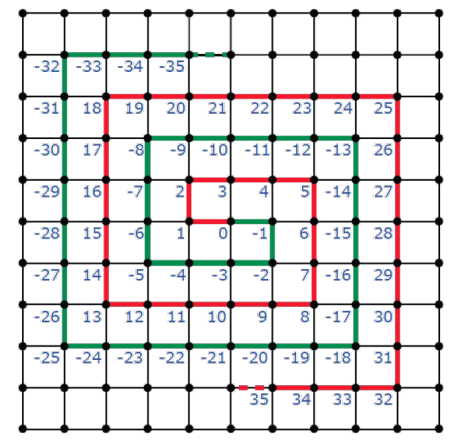
\includegraphics[width=0.35\textwidth]{Immagini/map_2to1_Ising.png}
    \caption{Mapping di un modello di Ising 2D su un modello di Ising 1D. Immagine da \cite{galliFSA}.}
    \label{fig: map_2to1_Ising}
\end{figure}

Sebbene si possa mappare il reticolo quadrato in una catena di spin, il motivo per cui tale reticolo lineare è ordinato a temperatura 
finita è da ricercare nel range dell'interazione. Nel caso del modello di Ising 1D con interazione fra primi vicini, la stessa è short 
range, poichè coinvolge solamente i siti adiacenti a quello preso in considerazione. Nel caso invece di catena di spin ottenuta come 
risultato del mapping di un reticolo quadrato in uno lineare, l'interazione è long-range, ed a ogni nuovo cambio di direzione delle 
spirali concentriche con cui si visitano tutti i siti reticolari tale lunghezza d'interazione aumenta. Nel caso della catena di 
spin ottenuta a partire da un reticolo quadrato anche i domain walls interagiscono fra loro con un potenziale di tipo long-range, andando 
ad invalidare il discorso fatto in precedenza e rendendo possibile una magnetizzazione non nulla anche per una catena di spin. 





\subsection{Fenomeni ad invarianza di scala}

La transizione di fase che avviene alla temperatura critica $T_c$ \eqref{eq: tc_Ising2D_Ons} è una transizione di fase continua. Una delle 
conseguenze della criticità è la perdita di un parametro di scala, nel senso che il sistema presenta cluster di spin di tutte le dimensioni. 
Chiaramente nel caso di una simulazione questa distribuzione sarà influenzata dalle dimensioni finite del reticolo considerato, dato che 
non è computazionalmente possibile lavorare nel limite termodinamico. Inoltre al punto critico il comportamento di un sistema è 
solitamente indipendente dai dettagli microscopici dello stesso, in quanto è determinato da poche caratteristiche quali

\begin{itemize}[label=$\diamond$] 
    \item la dimensionalità $d$ del sistema (per il modello di Ising 2D avremo $d\,=\,2$)
    \item il numero di componenti $n$ del parametro d'ordine
    \item il range delle interazioni microscopiche presenti fra i costituenti del sistema
\end{itemize}

Dato che il comportamento critico del sistema non ha alcuna dipendenza sui gradi di libertà microscopici dello stesso, è possibile mediante 
una tecnica di coarse graining rimuovere i gdL irrilevanti fino a quando si giunge alla lunghezza di correlazione. Tale metodo consiste 
nel dividere il reticolo in blocchi di dimensione inferiore rispetto a quella reticolare e sommare gli spin all'interno dei singoli cluster. 
Se il risultato dell'operazione precedente è positivo, il blocco verrà sostituito da un singolo spin orientato verso l'alto (+1), 
altrimenti da uno che punta verso il basso. Il modello risultante avrà di conseguenza un differente passo reticolare. Bisogna ora  
distinguere tre possibili scenari in base alla temperatura alla quale viene effettuata la simulazione.



\subsubsection{$T\,<\,T_c$}

Al di sotto della temperatura critica, il sistema è dotato di ordine a lungo raggio, ma dato che $T \neq 0$ sono presenti anche cluster 
di grandi dimensioni con spin orientati nella direzione opposta. Applicando in modo iterativo il metodo riportato in precedenza, la 
dimensione della cella unitaria aumenta e le fluttauazioni che sono di dimensione inferiore rispetto al passo reticolare scompaiono. 
Questo implica che il sistema diventa via via più ordinato e tende ad una configurazione con spin totalmente allineati tipica di 
$T\,=\,0$. In Figura \ref{fig: cg_2.0} è riportato un esempio di coarse graining applicato ad un reticolo di $10000 \times 10000$ 
spin, in cui per ogni mossa i sotto-blocchi che vengono presi in considerazione sono di dimensione $10 \times 10$. Si può osservare 
che applicando iterativamente l'algoritmo, le poche eccitazioni presenti nello stato di partenza vengono eliminate, giungendo ad un 
modello con spin completamente allineati. 



\subsubsection{$T\,>\,T_c$}

Al di sopra della temperatura critica, il sistema è disordinato e gli spin formano randomicamente cluster con orientazione verso 
l'alto oppure verso il basso. Ogni volta che viene effettuata una trasformazione, la lunghezza di correlazione diminuisce e i cluster 
diventano di dimensioni inferiori come se la temperatura stesse aumentando. Il sistema tende alla condizione di temperatura infinita, 
con cluster che coinvolgono un numero esiguo di momenti magnetici. In Figura \ref{fig: cg_3.0} è riportato un esempio di coarse graining 
applicato ad un reticolo di $10000 \times 10000$ spin, in cui per ogni mossa i sotto-blocchi che vengono presi in considerazione sono 
di dimensione $10 \times 10$. Si può osservare che applicando iterativamente l'algoritmo il reticolo continua a mantenere le caratteristiche 
tipiche dell'alta temperatura, ossia cluster di spin di piccole dimensioni.



\subsubsection{$T\,=\,T_c$}

Alla temperatura critica, i cluster sono di tutte le dimensioni, partendo da singoli spin per giungere ad un numero macroscopico di 
momenti magnetici coinvolti. In questo caso la lunghezza di correlazione è infinita e per iterazioni successive del metodo introdotto 
in precedenza non si ha alcun cambio nella distrubuzione delle dimensioni dei cluster. Il reticolo rimane a $T_c$, che risulta essere 
un punto fisso della funzione di coarse-graining. Chiaramente, gli altri punti fissi sono $T\,=\,0$ e $T\,=\,\infty$ a cui tendono 
tutti i sistemi che non si trovano in partenza al punto critico. Nella Figura seguente è possibile apprezzare l'applicazione della 
tecnica precedentemente esposta ad un sistema con $T \simeq T_c$, in cui una singola iterazione dell'algoritmo ha come unico effetto 
la cancellazione dei cluster di dimensione inferiore alla dimensione dei sotto-blocchi.


\vspace*{\fill}

\begin{tikzpicture}
    \node (img1) at (-1,0) {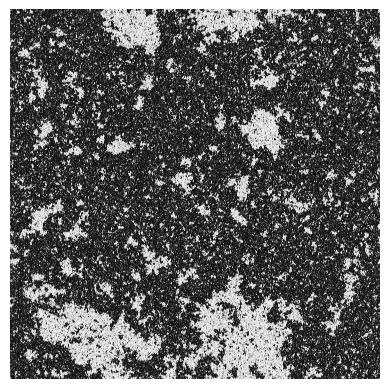
\includegraphics[width=0.4\textwidth]{Immagini/simIsing2D/cg/cg_10000_Tc.png}};
    
    \node (img2) at (7,0) {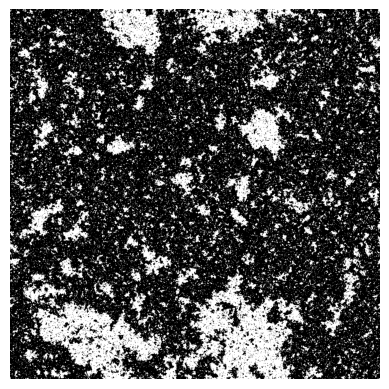
\includegraphics[width=0.4\textwidth]{Immagini/simIsing2D/cg/cg_1000_Tc.png}};
    
    \draw[->,thick] (img1.east)  -- node[above] {CG} (img2.west);

\end{tikzpicture}

\vspace*{\fill}


\vspace*{\fill}

\begin{figure}[htbp]
    \centering
    \begin{minipage}{0.45\textwidth}  
      \centering
      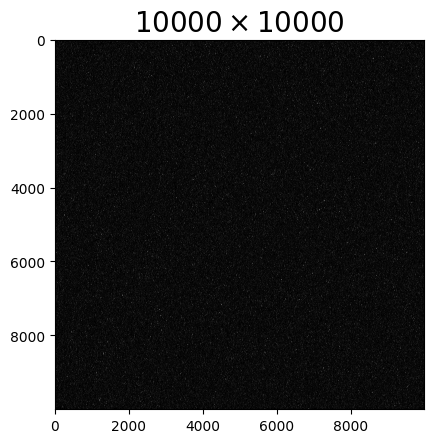
\includegraphics[page=1, width=\textwidth]{Immagini/simIsing2D/cg/cg_10000_2.0.png}
      \caption{Stato iniziale}
    \end{minipage}\hfill
    \begin{minipage}{0.45\textwidth}  
      \centering
      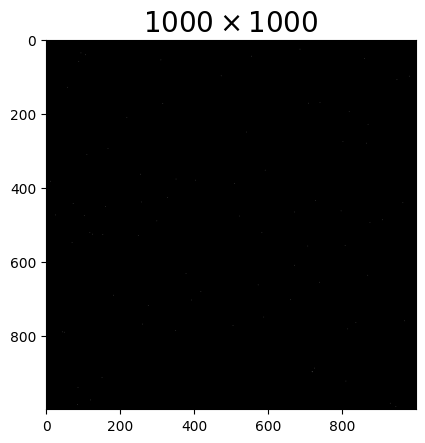
\includegraphics[page=1, width=\textwidth]{Immagini/simIsing2D/cg/cg_1000_2.0.png}
      \caption{Prima iterazione}
    \end{minipage}
    \vskip\baselineskip 
  
    \begin{minipage}{0.45\textwidth}  
      \centering
      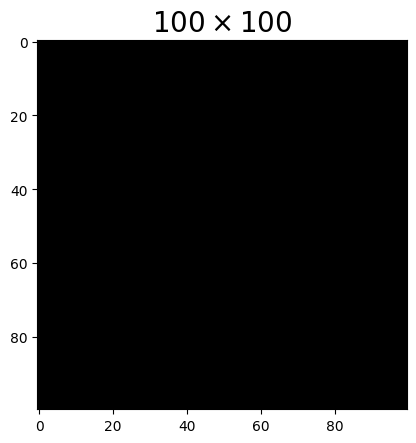
\includegraphics[page=1, width=\textwidth]{Immagini/simIsing2D/cg/cg_100_2.0.png}
      \caption{Seconda iterazione}
    \end{minipage}\hfill
    \begin{minipage}{0.45\textwidth}  
      \centering
      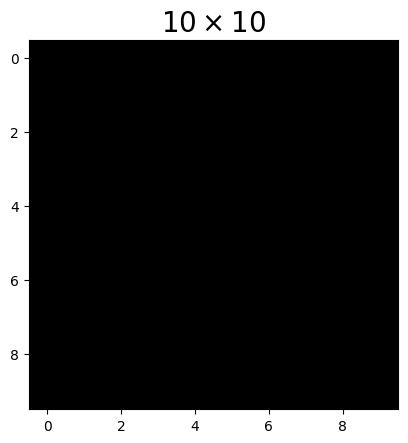
\includegraphics[page=1, width=\textwidth]{Immagini/simIsing2D/cg/cg_10_2.0.png}
      \caption{Terza iterazione}
    \end{minipage}

    \caption{Esempio di coarse-graining per un reticolo di $10000 \times 10000$ spin in equilibrio termodinamico alla 
    temperatura $T\,=\,2.0$. Ogni iterazione dell'algoritmo riduce di un fattore 10 il numero degli spin costituenti i lati 
    del quadrato.}
    \label{fig: cg_2.0}
\end{figure}

\vspace*{\fill}

\vspace*{\fill}

\begin{figure}[htbp]
    \centering
    \begin{minipage}{0.45\textwidth}  
      \centering
      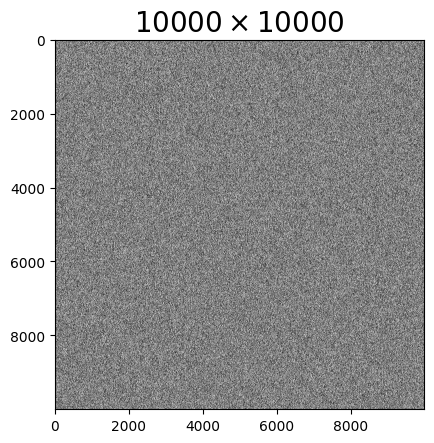
\includegraphics[page=1, width=\textwidth]{Immagini/simIsing2D/cg/cg_10000_3.0.png}
      \caption{Stato iniziale}
    \end{minipage}\hfill
    \begin{minipage}{0.45\textwidth}  
      \centering
      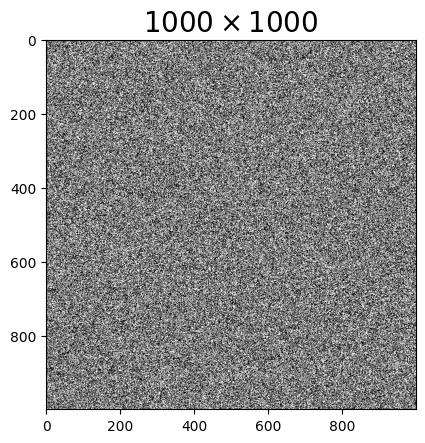
\includegraphics[page=1, width=\textwidth]{Immagini/simIsing2D/cg/cg_1000_3.0.png}
      \caption{Prima iterazione}
    \end{minipage}
    \vskip\baselineskip 
  
    \begin{minipage}{0.45\textwidth}  
      \centering
      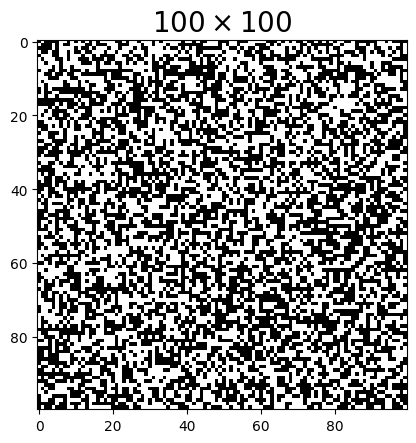
\includegraphics[page=1, width=\textwidth]{Immagini/simIsing2D/cg/cg_100_3.0.png}
      \caption{Seconda iterazione}
    \end{minipage}\hfill
    \begin{minipage}{0.45\textwidth}  
      \centering
      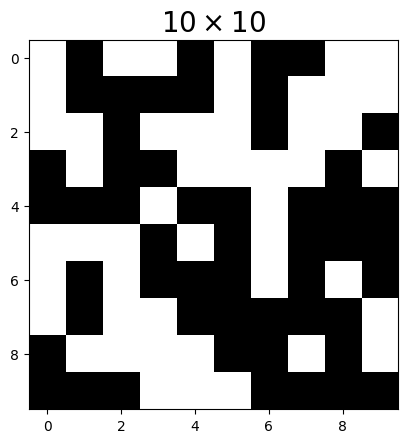
\includegraphics[page=1, width=\textwidth]{Immagini/simIsing2D/cg/cg_10_3.0.png}
      \caption{Terza iterazione}
    \end{minipage}

    \caption{Esempio di coarse-graining per un reticolo di $10000 \times 10000$ spin in equilibrio termodinamico alla 
    temperatura $T\,=\,3.0$. Ogni iterazione dell'algoritmo riduce di un fattore 10 il numero degli spin costituenti i lati 
    del quadrato.}
    \label{fig: cg_3.0}
\end{figure}

\vspace*{\fill}